% ==========================================
% BAB V RENCANA SELANJUTNYA
% Memakai kolom tabel Y dan Z yang didefinisikan pada Bab III.
% Isi bab ini mengikuti Proposal_TA_Konten.docx (revisi 18 November 2026).
% ==========================================
\cleardoublepage % memastikan bab baru dimulai di halaman ganjil (kanan)
\chapter{RENCANA SELANJUTNYA}
\label{chap:rencana-selanjutnya}

% ============================================================================================
% V.1 Rencana implementasi
% ============================================================================================
\section{Rencana Implementasi}
\label{sec:rencana-implementasi}
Bagian ini membahas rencana implementasi tugas akhir, yaitu membangun \textit{pipeline} eksperimen, beserta jadwal dan rinciannya.
Perkiraan jadwal pelaksanaan ditunjukkan pada Tabel~\ref{tab:jadwal}.
Rinciannya meliputi alat dan bahan, lingkungan dan konfigurasi pelaksanaan, serta perkiraan biaya.

\begin{table}[H]
  \centering
  \caption{Perkiraan jadwal pelaksanaan}
  \label{tab:jadwal}
  \footnotesize
  \begin{tabularx}{\textwidth}{| l | Y | Z{0.35\textwidth} |}
    \hline
    No. & Langkah & Perkiraan waktu \\
    \hline
    1 & Persiapan perekaman & Februari 2027 \\
    \hline
    2 & Perekaman data & Maret 2027 \\
    \hline
    3 & Prapemrosesan & Maret 2027 \\
    \hline
    4 & Model \textit{embedding} dan RCT & Maret 2027 \\
    \hline
    5 & SAE & Maret 2027 \\
    \hline
    6 & \textit{Adapter}, LLM, dan LoRA & April 2027 \\
    \hline
    7 & Pembanding & Mei 2027 \\
    \hline
    8 & Evaluasi & Mei 2027 \\
    \hline
    9 & Penulisan laporan & Juni 2027 \\
    \hline
  \end{tabularx}
\end{table}

\subsection{Alat dan Bahan}
\label{sec:alat-bahan}
Alat dan bahan yang diperlukan ditunjukkan pada Tabel~\ref{tab:alat-bahan}.

\begin{table}[H]
  \centering
  \caption{Alat dan bahan}
  \label{tab:alat-bahan}
  \footnotesize
  \begin{tabularx}{\textwidth}{| Z{0.22\textwidth} | Y |}
    \hline
    Komponen & Kebutuhan \\
    \hline
    Perangkat perekam EEG & Perekam EEG non-invasif dan portabel milik kampus. \\
    \hline
    Partisipan & Orang sehat sebanyak 10 orang, yang cukup untuk uji statistik pada pengujian lintas subjek. \\
    \hline
    Daftar kata atau frasa & 10 kata atau frasa berbahasa Inggris, dengan banyak percobaan untuk setiap kata. \\
    \hline
    Komputer pelatihan & Laptop pribadi dengan GPU untuk menjalankan Qwen3.5-9B secara lokal beserta pelatihan \textit{adapter} dan LoRA, dengan kuantisasi bila memori GPU tidak cukup. \\
    \hline
    Perangkat lunak & Python, MNE-Python, pyRiemann, sentence-transformers dengan model all-MiniLM-L6-v2, scikit-learn dan PyTorch, serta Transformers. \\
    \hline
  \end{tabularx}
\end{table}

\subsection{Lingkungan dan Konfigurasi}
\label{sec:lingkungan-konfigurasi}
Seluruh \textit{pipeline} dijalankan dalam satu lingkungan Python, dan versi setiap \textit{library} dicatat agar eksperimen dapat diulang.
Qwen3.5-9B dijalankan secara lokal dengan bobot yang dibekukan, dan hanya \textit{adapter} serta LoRA bila dipakai yang dilatih.
Setiap percobaan dijalankan dari satu berkas konfigurasi yang memuat pilihan memakai atau melewati RCT dan SAE, skema pengujian beserta pembagian data latih, validasi, dan uji, serta benih acak dan versi \textit{library}.
Pengaturan yang belum pasti, yaitu jenis model regresi, nilai $K$ pada \textit{adapter}, lebar SAE, dan jenis model klasifikasi pembanding, dipilih dengan data validasi.
Hasil setiap percobaan dicatat bersama konfigurasinya.

\subsection{Biaya}
\label{sec:biaya}
Rincian biaya ditunjukkan pada Tabel~\ref{tab:biaya}.

\begin{table}[H]
  \centering
  \caption{Perkiraan biaya}
  \label{tab:biaya}
  \footnotesize
  \begin{tabularx}{\textwidth}{| Z{0.25\textwidth} | Y | Z{0.2\textwidth} |}
    \hline
    Komponen & Keterangan & Perkiraan biaya \\
    \hline
    Perangkat EEG & Dipinjam dari kampus. & Rp0 \\
    \hline
    Kompensasi partisipan & 10 partisipan, masing-masing 1 sesi, Rp50.000 per sesi. & Rp500.000 \\
    \hline
    Komputasi GPU & Memakai laptop pribadi. & Rp0 \\
    \hline
    Perangkat lunak dan model & Python, \textit{library} pendukung, dan Qwen3.5-9B yang bersumber terbuka. & Rp0 \\
    \hline
    \textbf{Total} & & \textbf{Rp500.000} \\
    \hline
  \end{tabularx}
\end{table}

% ============================================================================================
% V.2 Desain pengujian dan evaluasi
% ============================================================================================
\section{Desain Pengujian dan Evaluasi}
\label{sec:rencana-pengujian}
Bagian ini membahas rancangan pengujian dan evaluasi untuk menjawab rumusan masalah dan menguji hipotesis.
Pembahasan terdiri dari skema validasi, yaitu cara data dibagi dan pengaturan dipilih, serta evaluasi, yaitu cara performa diukur dan diuji secara statistik.

\subsection{Validasi}
\label{sec:validasi}
Pengujian dilakukan pada dua skema, yaitu per subjek dan lintas subjek.
Data dibagi menjadi data latih untuk melatih model, data validasi untuk memilih pengaturan, dan data uji yang hanya dipakai sekali untuk laporan akhir.

Pada pengujian per subjek, data setiap subjek dibagi acak dengan jumlah percobaan yang seimbang untuk setiap kata menjadi data latih, validasi, dan uji.
Model dilatih dan diuji pada subjek yang sama.
Pada pengujian lintas subjek, setiap subjek bergantian menjadi subjek uji dan model dilatih pada semua subjek lainnya.
Sebagian percobaan dari subjek-subjek pelatihan, misalnya 15 persen, dipakai sebagai data validasi.
Data dan label subjek uji tidak dipakai sama sekali pada pelatihan, dan pada RCT rata-rata subjek uji dihitung hanya dari rekamannya sendiri.
Dengan 10 subjek, terdapat 10 putaran.
Pembagian data pada kedua skema ditunjukkan pada Gambar~\ref{fig:validasi}.

\begin{figure}[t]
  \centering
  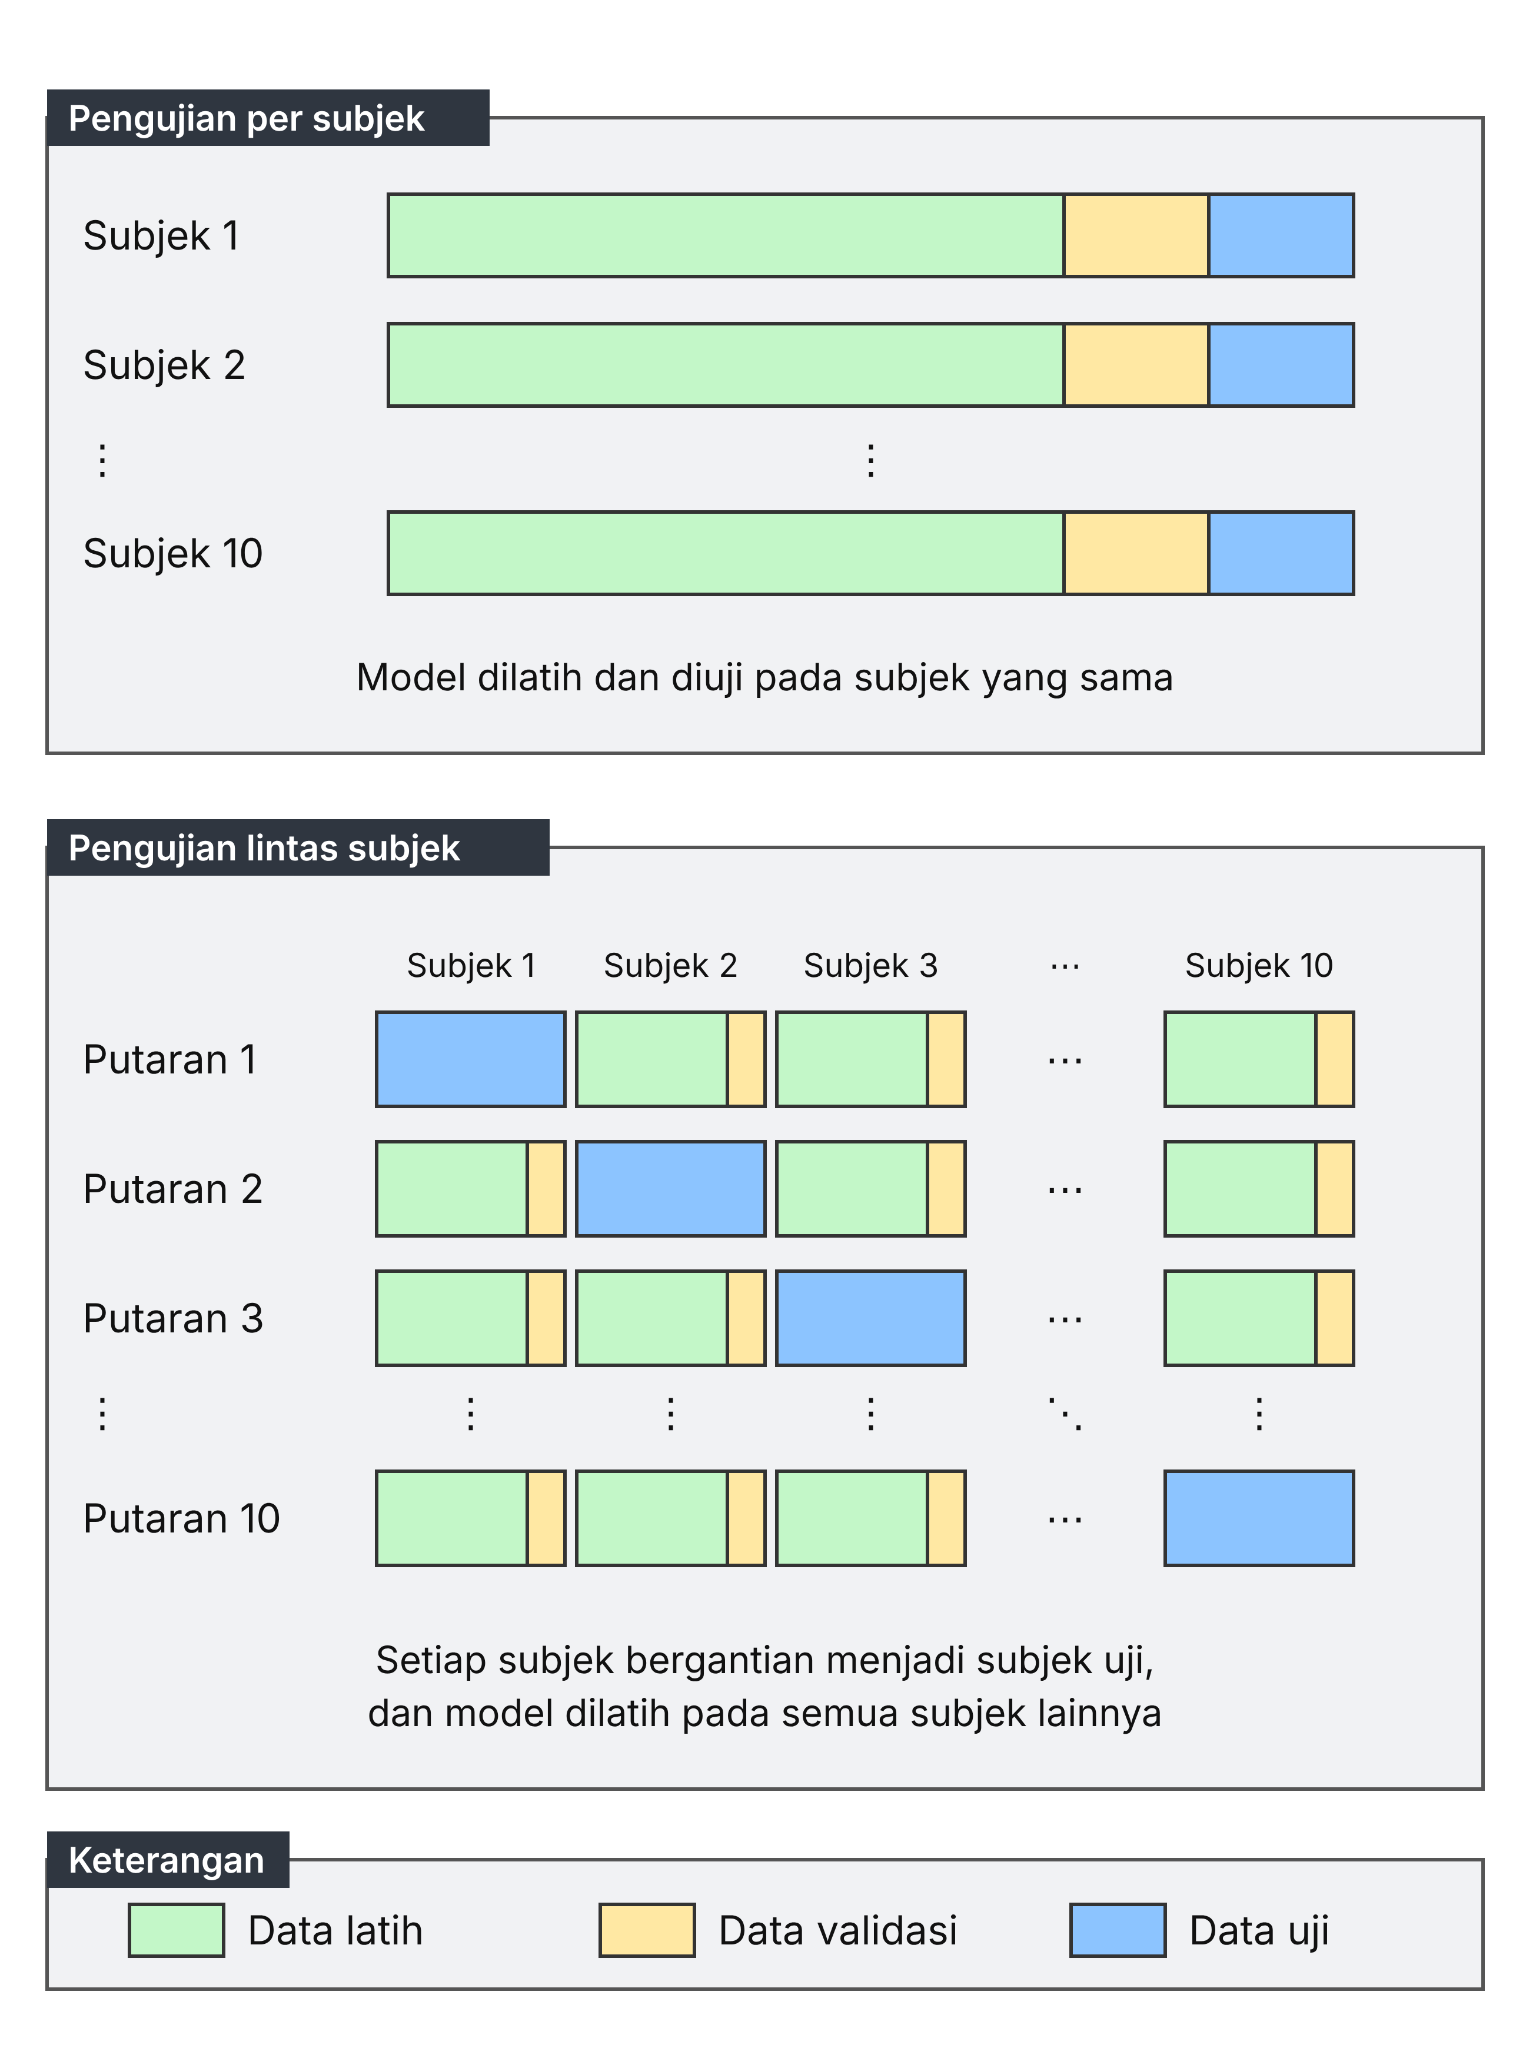
\includegraphics[width=0.75\textwidth]{images/gambar_V_validasi.png}
  \caption{Pembagian data latih, validasi, dan uji pada pengujian per subjek dan lintas subjek dengan 10 subjek}
  \label{fig:validasi}
\end{figure}

Data validasi dipakai untuk memilih pengaturan yang belum pasti, yaitu jenis model regresi, nilai $K$ pada \textit{adapter}, lebar SAE, dan jenis model klasifikasi pembanding.
Setiap konfigurasi dijalankan dengan beberapa benih acak, dan performa satu subjek adalah rata-rata dari benih-benih tersebut, dilaporkan beserta simpangan bakunya.
Pembagian data dan benih acak dibuat sama untuk semua konfigurasi sehingga perbedaan performa hanya berasal dari perbedaan konfigurasinya.

\subsection{Evaluasi}
\label{sec:evaluasi}
Performa keluaran berupa kata diukur dengan \textit{balanced accuracy}, dan keluaran berupa deretan kata dengan BERTScore \textit{recall}.
Tingkat tebakan acak untuk keluaran berupa kata adalah satu dibagi jumlah kata atau frasa pada \textit{dataset}, yaitu 10 persen untuk 10 kata atau frasa.
Sebagai analisis tambahan dilaporkan performa per kata dan matriks kebingungan (\textit{confusion matrix}), yaitu tabel yang menunjukkan kata mana yang sering tertukar dengan kata mana.

Setiap hipotesis diuji dengan taraf signifikansi 0,05.
Hipotesis 1 membandingkan performa model dengan tingkat tebakan acak menggunakan uji proporsi satu arah.
Percobaan uji dari semua subjek digabung untuk uji ini, dan karena percobaan dari subjek yang sama tidak sepenuhnya saling bebas, performa setiap subjek juga dilaporkan.
Hipotesis 2 membandingkan performa dengan dan tanpa RCT, keduanya tanpa SAE, pada pengujian lintas subjek menggunakan uji Wilcoxon berpasangan dua arah.
Setiap subjek uji memberikan satu pasangan performa, yaitu performanya dengan dan tanpa RCT, sehingga dengan 10 subjek terdapat 10 pasangan.
Selain nilai $p$, dilaporkan selisih median performa kedua cara agar besar perbedaannya terlihat.

Perbandingan dengan pendekatan klasifikasi dinilai sesuai ukuran keberhasilan ketiga pada Subbab~\ref{sec:tujuan}.
Model klasifikasi pembanding dilatih pada data latih yang sama dan dinilai dengan \textit{balanced accuracy} pada data uji dan pembagian data yang sama dengan keluaran LLM.
Setiap subjek uji memberikan satu pasangan performa, yaitu performa keluaran LLM dan performa model klasifikasi, yang diuji dengan uji Wilcoxon berpasangan dua arah dengan 10 pasangan.
Pencarian kata terdekat dinilai dengan cara yang sama dan dilaporkan sebagai pembanding tambahan.
Hasil juga dilaporkan berdampingan dengan metode klasifikasi pada penelitian terdahulu, dengan catatan bahwa data dan tugasnya berbeda sehingga perbandingan ini hanya bersifat rujukan.
Skor BERTScore \textit{recall} keluaran berupa deretan kata dilaporkan berdampingan dengan BERTScore Thought2Text sebesar 0,88 sampai 0,89 \parencite{mishra2025}, dengan catatan yang sama.

Hipotesis 1 diuji pada konfigurasi dengan performa validasi tertinggi, sedangkan semua konfigurasi tetap dilaporkan.
Pengaruh SAE dilaporkan secara deskriptif karena tidak menjadi hipotesis.
Sebagai rujukan, performa dibandingkan dengan ambang sekitar 70 persen yang dianggap layak untuk penerapan nyata \parencite{lopezbernal2022}, dan ambang ini tidak menjadi syarat keberhasilan.

% ============================================================================================
% V.3 Analisis risiko dan mitigasi
% ============================================================================================
\section{Analisis Risiko dan Mitigasi}
\label{sec:rencana-risiko}
Risiko yang mungkin muncul beserta tindakan selanjutnya bila terjadi ditunjukkan pada Tabel~\ref{tab:risiko}.

\begin{table}[H]
  \centering
  \caption{Analisis risiko dan mitigasi}
  \label{tab:risiko}
  \footnotesize
  \begin{tabularx}{\textwidth}{| l | Z{0.2\textwidth} | Z{0.2\textwidth} | Y |}
    \hline
    ID & Risiko & Dampak & Mitigasi dan tindakan selanjutnya \\
    \hline
    R01 & Persetujuan etik atau perekrutan partisipan terlambat & Perekaman data mundur & Pengajuan dilakukan sejak awal. Selama menunggu, \textit{pipeline} dikembangkan dan diuji dengan data sintetis yang kecil. \\
    \hline
    R02 & Partisipan atau percobaan kurang dari rencana & Uji statistik lemah & Menambah sesi dan partisipan. Bila subjek tetap kurang, hasil dilaporkan secara deskriptif disertai catatan bahwa uji tidak dapat dilakukan. \\
    \hline
    R03 & Sinyal banyak \textit{noise} & Performa mendekati tebakan acak & Protokol perekaman menyertakan jeda dan instruksi untuk meminimalkan gerakan. Kriteria pembuangan percobaan yang banyak \textit{noise} ditetapkan sebelum melihat hasil. \\
    \hline
    R04 & Performa mendekati tebakan acak pada semua konfigurasi & Hipotesis 1 tidak terpenuhi & Hasil tetap dilaporkan sebagai temuan. Penyebab ditelusuri tahap demi tahap, dimulai dari model regresi, lalu skema per subjek sebelum lintas subjek. \\
    \hline
    R05 & Qwen3.5-9B tidak muat pada GPU yang tersedia & Pelatihan \textit{adapter} dan LoRA tidak dapat dijalankan & Memakai kuantisasi, ukuran \textit{batch} kecil, atau model sumber terbuka yang lebih kecil. \\
    \hline
    R06 & \textit{Adapter} atau LoRA menghafal data latih karena data sedikit & Performa latih tinggi tetapi performa uji rendah & Menjaga $K$ tetap kecil, berhenti pelatihan berdasarkan data validasi, dan memakai LoRA hanya bila \textit{adapter} saja belum cukup. \\
    \hline
    R07 & Keluaran LLM tidak konsisten, misalnya berupa kalimat panjang & Penilaian tidak adil & Memakai perintah teks yang tetap dan membatasi panjang keluaran. Keluaran berupa kata yang tidak sama dengan label dinilai salah. \\
    \hline
    R08 & RCT atau SAE tidak meningkatkan performa & Hipotesis 2 tidak terbukti, atau SAE tidak berguna & Hasil dilaporkan apa adanya. \\
    \hline
    R09 & Kebocoran data tidak sengaja & Performa tampak lebih tinggi dari seharusnya & Data uji dan label subjek uji dipisahkan dari pelatihan sejak pembagian data, dan rata-rata RCT subjek uji dihitung tanpa label. \\
    \hline
    R10 & Hasil tidak dapat diulang & Hasil tidak dapat diverifikasi & Mencatat benih acak, versi \textit{library}, dan konfigurasi, serta memakai mode deterministik pada PyTorch bila tersedia. \\
    \hline
  \end{tabularx}
\end{table}
